\documentclass[dvipdfmx,uplatex,11pt]{jabstract}

%%% font の指定
%%% 特にローカルで文字化けするときに 環境に合わせて選んでください
%%% http://ctan.math.illinois.edu/language/japanese/pxchfon/pxchfon.pdf
%%%
%%%以下では
%%% texlive2020で公式に取り込まれた(という)haranoaji をしてしています

\usepackage[haranoaji]{pxchfon} % 原の味 fontを使う.info/texlive2020

%\usepackage[noembed]{pxchfon} % fontを埋め込まない.info/texlive2020
%\usepackage[ipa]{pxchfon} % IPA fontを使う. info/texlive2020
%\usepackage[ipaex]{pxchfon} % IPAex fontを使う.info/texlive2020
%\usepackage[ms]{pxchfon} % MS fontを使う.info/texlive2020
% 昨年までの環境 texlive2019f3
%\usepackage[noto-jp]{pxchfon} % noto font jpを使う.texlive2019f3

\usepackage[dvipdfmx]{graphicx}
\usepackage{bmpsize}
\usepackage[outdir=./]{epstopdf}
\usepackage[fleqn]{amsmath}

\jtitle{タイトルtext\\長い場合}
\jauthor{自分の名前}
\jaffiliation{情報工学分野}%{情報工学科}
\jteacher{指導教員名}

\begin{document}
\maketitle

\begin{multicols}{2}
  
\section{はじめに}
 現在一般的にプレイされているゲームでは、ゲーム世界のオブジェクトの温度を感じることはまだできない。ゲームで温度を表現する方法のひとつに、結露を利用する方法がある。結露とは、空気中の水蒸気が液体の水滴に変わるプロセスのことです。これは、空気が露点以下に冷やされたときに起こる。
 結露は、物体が低温であることを示すために使うことができる。例えば、寒い環境で息を吐くと、人の息が空気中で結露したり、冷たい飲み物の表面に結露が生じたりする。ゲームで温度を表現するために結露を使用すると、ゲーム体験をよりリアルにすることができる。

\section{IDマップ}
 IDマップは2次元の配列で、各座標における水滴の有無を格納する。配列のサイズは高さマップのサイズと同じである。配列の各要素は0または1で、0は水滴がないことを表し、1は水滴があることを表す。

\section{ハイトマップ}
 ハイトマップは、水滴の高さを表すグレースケール画像である。OpenCVを使用して生成され、法線マップを計算するための2Dテクスチャとして読み込まれる。ハイトマップは半球の形状に基づいており、水滴の中心から端に向かって高さが徐々に低くなっている。

\section{法線マップ}
法線マップは、水滴表面の各ピクセルの法線ベクトルを表すために使用される。法線ベクトルは表面に垂直で、外側を指す。法線マップは、ハイトマップから導関数を計算することによって作成される。この計算はGLSL(OpenGL Shading Language)で行われ、結果は保存されず、代わりにスネルの法則を使用して光の屈折を計算するために使用される。

\section{環境マップ}
環境マップは、周囲の環境を表現するために使用されるパノラマ画像である。環境マップはGPUに読み込まれ、水滴表面での光の屈折を計算するために使用される。この結果、よりリアルで視覚的に魅力的な結果が実現した。

\section{研究結果}
 現在の実装では、正しい屈折率で水滴を作成することに成功しているが、ハイトマップに2D画像テクスチャを使用しているため、結果はピクセル化されている。テクスチャ画像の解像度を上げれば結果の品質は向上しますが、実行時間も長くなる。
 将来には、以下のような実装を計画している: 
- フレネル反射を計算し、結果にリアリズムを加える。
- フレームごとにハイトマップテクスチャを更新し、アニメーション効果を作成する。
これらの改善により、結露シミュレーションはよりリアルで視覚的に魅力的なものになると思う。

\section{おわりに}
この方法は、テクスチャのみを使用することで、結露効果を比較的効率的にシミュレートしている。しかし、よりリアルな結果を得るためには、水滴の3Dモデルを使用することで、レンダリングシーンに奥行きが出ると思う。
% \begin{align*}
%   y &= ax^2 + bx + c\\
%   z &= ax^3 + bx^2 + cy^2 + d
% \end{align*}
% などを効果的に使う必要もあるだろう。

% \subsection{サブセクション}
% 必要に応じてサブセクションを設ける。しかし、紙面も限られているので本当
% にサブセクションが必要かどうかは、今一度考えてみるといいだろう。サブセ
% クションにせずとも、適切に段落分けすることで、十分読みやすい文章にする


% \begin{tablehere}
%   \caption{表の挿入例}
%   \label{tab:sample}
%   \begin{tabular}{|c|c|c|}
%     \hline
%     & jarticle & jpreprint\\
%     \hline
%     一段に収まる図 & figure環境 & figurehere環境\\
%     \hline
%     紙幅一杯の図 & figure*環境 & figure*環境\\
%     \hline
%     一段に収まる表 & table環境 & tablehere環境\\
%     \hline
%     紙幅一杯の表 & table*環境 & table*環境\\
%     \hline
%   \end{tabular}
% \end{tablehere}

% \begin{figurehere}
%   \centering
% %  \scalebox{0.5}{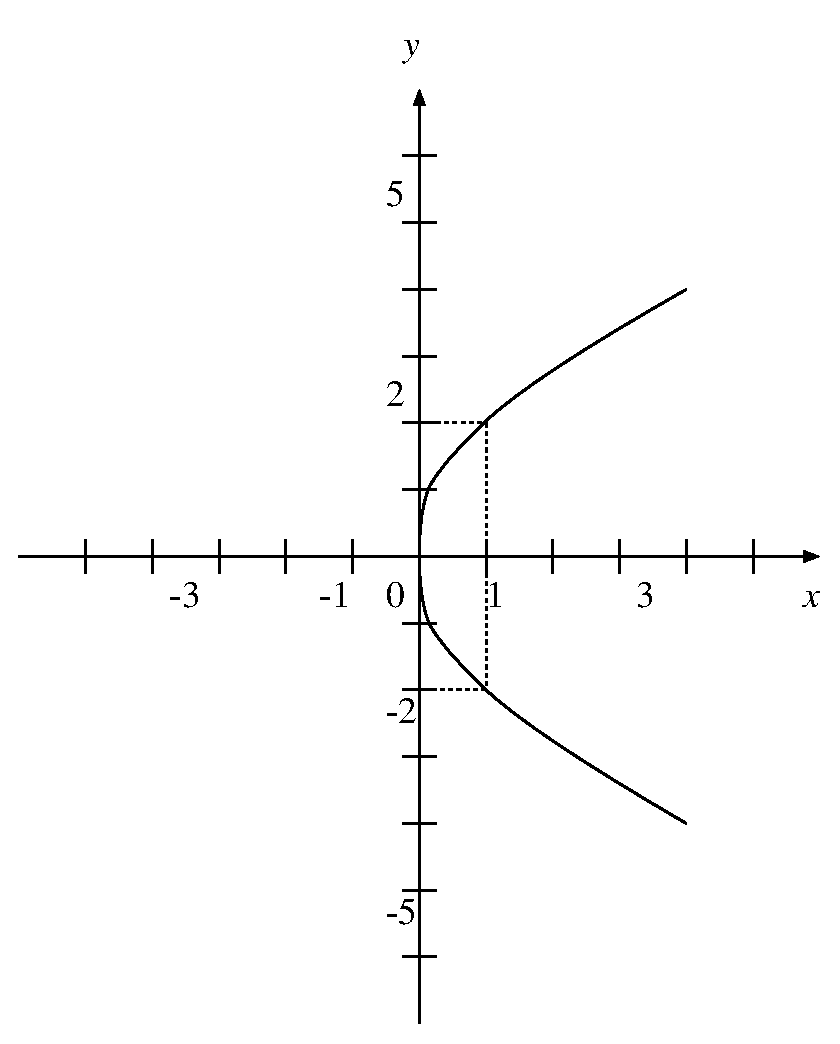
\includegraphics[bb= 0 0 1382 734,width=20cm]{sample.eps}}
%   \scalebox{0.5}{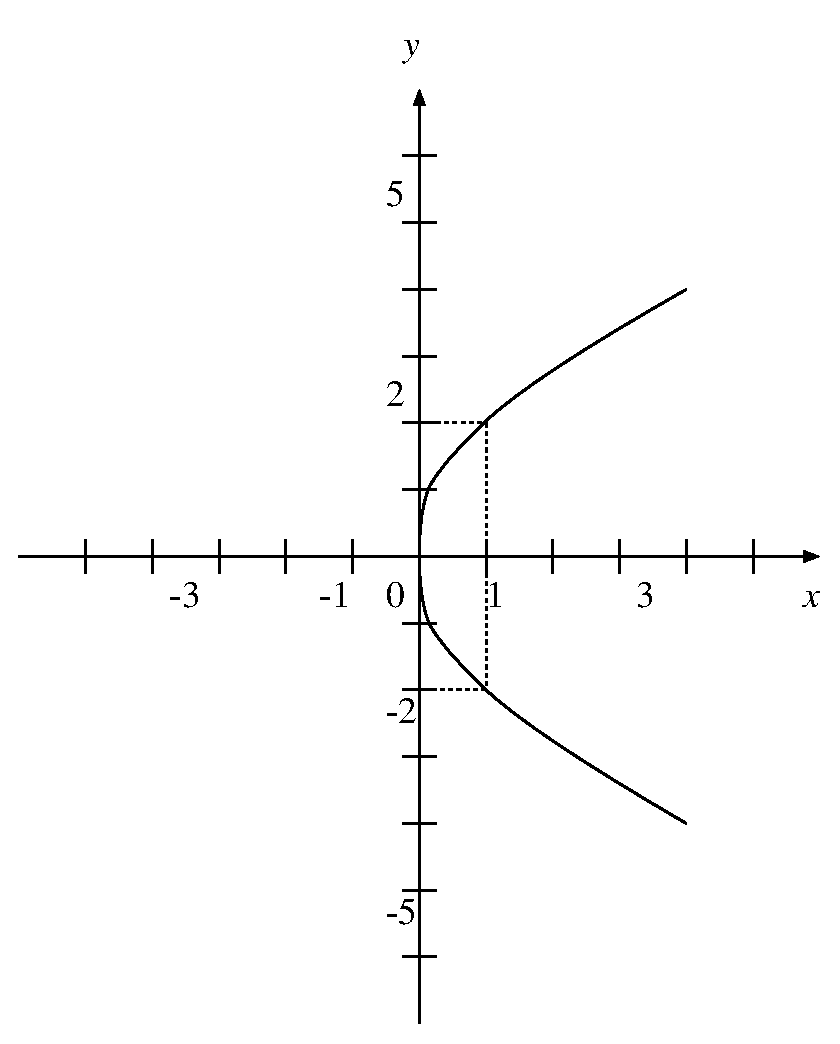
\includegraphics[]{sample.eps}}
%   \caption{図の挿入例}
%   \label{fig:sample}
% \end{figurehere}

% \section{次のセクション}
% 中間発表の場合は進捗状況や今後の方向性、進め方など、本発表の場合は自分
% の研究の核心部分や実験などがこのあたりに来ることになるだろう。

% \begin{enumerate}
% \item あれ
% \item これ
% \item それ
% \item どれ
% \end{enumerate}

% 箇条書きは紙面を食うので、必要性を慎重に考えなければならない。

% \section*{おわりに}
% 最後に全体をまとめ、自分の研究の成果と課題をはっきりさせることが肝心と
% なる。文章全体の印象を左右することにもなるので、ここも気は抜けない。

%
% 以下に文献を書きます。
% 最後の section との間に必ず空行を開けること

{\small
\begin{thebibliography}{99}
\end{thebibliography}
}

\end{multicols}

\end{document}
